\chapter{Examples}
\label{ch:Examples}
Each chapter automatically starts on a new page.
 

\section{Section}
This is the start of a new section.
 

\subsection{Subsection}
This is the start of a new subsection.
 

\subsubsection{Subsubsection}
This is the start of a new subsubsection. Subsubsections don't get a number and don't appear in the table of contents.
 

\paragraph{A paragraph} starts with words set in bold letters (try to avoid this).
 

\subparagraph{A subparagraph} starts with words set in sans serif bold letters (try to avoid this).
 

\section{Pages with figures}
 

\begin{figure}[htbp]
    \centering
    
\includegraphics[width=0.6\columnwidth]{figures/TUBAF_Logo_blau.png}
    \caption{TUBAF Logo.}
    \label{fig:TUBAF_Logo_1}
\end{figure}

Figure \ref{fig:TUBAF_Logo_1} shows the TUBAF logo.
 
\begin{figure}[htbp]
    \centering
    
\includegraphics[width=0.3\columnwidth]{figures/TUBAF_Logo_blau.png}
    \caption{TUBAF Logo. And a very long caption.  And a very long caption.  And a very long caption.  And a very long caption.  And a very long caption.  And a very long caption.  And a very long caption.  And a very long caption.}
    \label{fig:TUBAF_Logo_2}
\end{figure}

Figure \ref{fig:TUBAF_Logo_2} shows the TUBAF logo.

 

\begin{figure}[htbp]
     \centering
     \begin{subfigure}[t]{0.55\textwidth}
         \centering
         
\includegraphics[width=\textwidth]{figures/TUBAF_Logo_blau.png}
         \caption{The official TUBAF logo.}
         \label{fig:TUBAF}
     \end{subfigure}
     \hfill
     \begin{subfigure}[t]{0.33\textwidth}
         \centering
         
\includegraphics[width=\textwidth]{figures/imfd_logo_trans.png}
         \caption{The IMFD logo.}
         \label{fig:IMFD}
     \end{subfigure}
     \caption{A figure with two subfigures. The subcaptions have their own labels.}
     \label{fig:TUBAF-IMFD2}
\end{figure}
In Figure \ref{fig:TUBAF-IMFD2} two subfigures are included. \ref{fig:TUBAF} and \ref{fig:IMFD} are references.

\section{Pages with tables}
 
\begin{table}[htbp]
    \centering
    \captionabove{A very simple table.}
    \label{tab:simple}
    \begin{tabular}{c|ccc}
        %\toprule
        \hline
           & i & j & k \\
        %\midrule
        \hline
         1 & d & e & f \\
         2 & g & h & i \\
        %\bottomrule
        \hline
    \end{tabular}
\end{table}

Table \ref{tab:simple} shows a very simple table. Figures and tables are always centered. If the captions are longer than a single line they will stretch over the whole textwidth.

Use \verb|\captionabove{caption text}| to get the skip between caption and table.

\section{Equations}
\subsection{Problem 1}
\begin{equation}
E=mc^2
\label{eq:Einstein1}
\end{equation}
Equation \eqref{eq:Einstein1} shows\footnote{Footnote} ...

\clearpage
Therein, $\boldsymbol{Q}^{\star}(\tau)\!:\mathfrak{T}\to SO(d)$ is a \emph{(proper) orthogonal} second-order tensor, i.e., $\mathrm{det}(\boldsymbol{Q}^{\star})\!=\!1$, and $a\!\in\!\mathbb{R}$ denotes a \emph{time-shift}. Any \emph{change of observers} (sometimes called \emph{change of frame of reference}) $\tilde{\mathfrak{O}}\circ\mathfrak{O}^{-1}\!:\mathbb{R}^{d}\times\mathbb{R}\to\mathbb{R}^{d}\times\mathbb{R}$ is therefore called \emph{objective}, if it fulfills . If $\mathfrak{O}$ and $\tilde{\mathfrak{O}}$ have chosen respective reference configurations $\boldsymbol{\varphi}^{\star}_{\tau_{0}}$ and $\tilde{\boldsymbol{\varphi}}^{\star}_{\tau_{0}}$,  an be rewritten as
\begin{align}
	\tilde{\boldsymbol{\varphi}}_{\tau}\big(\tilde{\boldsymbol{\varphi}}^{\star}_{\tau_{0}}(\mathcal{X})\big) - \tilde{\boldsymbol{\varphi}}_{\tau}\big(\tilde{\boldsymbol{\varphi}}^{\star}_{\tau_{0}}(\mathcal{X}_{0})\big) = \boldsymbol{Q}^{\star}(\tau)\cdot\big[\boldsymbol{\varphi}_{\tau}\big(\boldsymbol{\varphi}^{\star}_{\tau_{0}}(\mathcal{X})\big) - \boldsymbol{\varphi}_{\tau}\big(\boldsymbol{\varphi}^{\star}_{\tau_{0}}(\mathcal{X}_{0})\big)\big] \ ,
\end{align}
with $\tilde{\boldsymbol{\varphi}_{\tau}}\!:=\!\tilde{\boldsymbol{\varphi}}^{\star}_{\tau}\circ\tilde{\boldsymbol{\varphi}}^{\star-1}_{\tau_{0}}$ and $\boldsymbol{\varphi}_{\tau}\!:=\!\boldsymbol{\varphi}^{\star}_{\tau}\circ\boldsymbol{\varphi}^{\star-1}_{\tau_{0}}$. Making use of definition , the derived observer transformation rule can be simplified further if $\mathfrak{O}$ and $\tilde{\mathfrak{O}}$ agree on the same reference configuration, since then, by identifying $\!\boldsymbol{\varphi}^{\star}_{\tau_{0}}(\mathcal{X})\!=\!\tilde{\boldsymbol{\varphi}}^{\star}_{\tau_{0}}(\mathcal{X})\!=:\!\boldsymbol{X}$, $\!\boldsymbol{\varphi}^{\star}_{\tau_{0}}(\mathcal{X}_{0})\!=\!\tilde{\boldsymbol{\varphi}}^{\star}_{\tau_{0}}(\mathcal{X}_{0})\!=:\!\boldsymbol{X}_{0}$, $\tilde{t}(\tau)\!=:\!\tilde{t}$ as well as $t(\tau)\!=:\!t$, it follows that
\begin{align}
	\tilde{\boldsymbol{\varphi}}\big(\boldsymbol{X},\tilde{t}\;\!\big) - \tilde{\boldsymbol{\varphi}}\big(\boldsymbol{X}_{0},\tilde{t}\;\!\big) = \boldsymbol{Q}^{\star}(\tau)\cdot\big[	\boldsymbol{\varphi}\big(\boldsymbol{X},t\big) - \boldsymbol{\varphi}\big(\boldsymbol{X}_{0},t\big) \big] \ .
\end{align}
Rearranging the terms now finally results in the well-known equation for the \emph{change of current configuration} based on a change of observers
\begin{align}
		\tilde{\boldsymbol{\varphi}}\big(\boldsymbol{X},\tilde{t}\;\!\big) = \boldsymbol{Q}(t)\cdot\boldsymbol{\varphi}(\boldsymbol{X},t) + \boldsymbol{c}(\boldsymbol{X}_{0},t) \ ,
\end{align}
in which $\boldsymbol{c}\;\!(\boldsymbol{X}_{0},t)\!:=\!\tilde{\boldsymbol{\varphi}}(\boldsymbol{X}_{0},t+a) - \boldsymbol{Q}(t)\cdot\boldsymbol{\varphi}(\boldsymbol{X}_{0},t)$ and $\boldsymbol{Q}(t)\!:=\!\boldsymbol{Q}^{\star}(t^{-1}(t))$. The more familiar formulations of this equation is known from the literature as $\tilde{\boldsymbol{x}}\!=\!\boldsymbol{Q}(t)\cdot\boldsymbol{x} + \boldsymbol{c}(t)$, despite the fact that it loses some important details. Note that $\boldsymbol{X}_{0}$ is conventionally identified as the \emph{fixed} origin $\boldsymbol{o}$ of the reference configuration, so that $\boldsymbol{c}$ is represented as a function of time only. Fixing one specific $\boldsymbol{X}_{0}$, which is of course independent on $\boldsymbol{X}$, the deformation gradient consequently transforms under a change of observers as
\begin{align}
	\tilde{\boldsymbol{F}}(\boldsymbol{X},t):=\partial_{\boldsymbol{X}}\tilde{\boldsymbol{\varphi}}(\boldsymbol{X},t) = \boldsymbol{Q}(t)\!\cdot\!\partial_{\boldsymbol{X}}\boldsymbol{\varphi}(\boldsymbol{X},t) = \boldsymbol{Q}(t)\!\cdot\!\boldsymbol{F}(\boldsymbol{X},t) \ .
\end{align}
In contrast, the \textsc{Green} strain tensor remains constant during an observer transformation, since $\tilde{\boldsymbol{E}}\!:=\!\frac{1}{2}[\tilde{\boldsymbol{F}}{^{\mathrm{T}}}\!\cdot\tilde{\boldsymbol{F}} - \boldsymbol{I}]\!=\!\frac{1}{2}[\boldsymbol{F}^{\mathrm{T}}\!\cdot\boldsymbol{Q}^{T}\!\!\cdot\boldsymbol{Q}\cdot\boldsymbol{F} - \boldsymbol{I}]\!=\!\boldsymbol{E}$ due to the orthogonality $\boldsymbol{Q}^{\mathrm{T}}\!\cdot\boldsymbol{Q}\!=\!\boldsymbol{I}$. Accordingly, given some arbitrary tensor-valued field quantity $\boldsymbol{\xi}\!:\mathcal{B}\times\mathcal{T}\to\mathbb{R}^{d\;\!\otimes\;\!m}$, that is defined over the reference configuration $\mathcal{B}$ and time range $\mathcal{T}$ of a specific observer, its transformation behavior under a change of observers strictly depends on its mathematical structure\footnote{The terminology \emph{production volume density} implies that, in the absence of supply and flux contributions, any \emph{scalar} field quantity $\xi$ is only allowed to increase, so that the production volume density must be non-negative, i.e., $p_{\xi}\!\geq\!0$. However, considering tensor-valued field quantities, it is not possible to decide whether or not a quantity $\boldsymbol{\xi}\!\in\!\mathbb{R}^{d\;\!\otimes\;\!m}$ is increasing, since $\mathbb{R}^{d\;\!\otimes\;\!m}$ is not equipped with an \emph{order relation}. This \emph{issue} can be resolved by defining a differentiable \emph{norm} $\mathcal{N}\!:\mathbb{R}^{d\;\!\otimes\;\!m}\;\!\to\mathbb{R}^{+}$ and requiring that $\forall\!\;\boldsymbol{X}\!\in\!\mathcal{B}$ and $\forall\;\!t\!\in\!\mathcal{T}\!:\;\!\partial_{\boldsymbol{\xi}}\mathcal{N}(\boldsymbol{\xi})\!\cdot\!\boldsymbol{p}_{\boldsymbol{\xi}}\!\geq\!0$.}, which is determined by the image $\mathrm{im}_{\boldsymbol{\xi}}(\mathcal{B}\times\mathcal{T})\subset\mathbb{R}^{d\;\!\otimes\;\!m}$. More specifically, if $\mathfrak{O}$ refers to the tangent spaces $T_{\boldsymbol{X}}\mathcal{B}$ and $T_{\boldsymbol{x}}\;\!\mathcal{B}_{t}$ in its reference and current configuration, respectively, a different observer $\tilde{\mathfrak{O}}$ is equipped with $T_{\tilde{\boldsymbol{X}}}\tilde{\mathcal{B}}$ and $T_{\tilde{\boldsymbol{x}}}\;\!\tilde{\mathcal{B}}_{t}$ due to the change of frame of reference. Therein, $\mathfrak{O}$ and $\tilde{\mathfrak{O}}$ are free to chose their reference configuration independently, so that in general $\mathcal{B}\!\neq\!\tilde{\mathcal{B}}$. Now, if the image of $\boldsymbol{\xi}$ observed by $\mathfrak{O}$ is identified as 
\begin{align}
	\mathrm{im}_{\boldsymbol{\xi}}(\mathcal{B}\times\mathcal{T})\!=\!\mathrm{Lin}(T_{\boldsymbol{X}}\mathcal{B}\otimes...\otimes T_{\boldsymbol{X}}\mathcal{B} \otimes T_{\boldsymbol{x}}\;\!\mathcal{B}_{t}\otimes ... \otimes T_{\boldsymbol{x}}\;\!\mathcal{B}_{t}, \mathbb{R}),
\end{align}
in which $n$ copies of $T_{\boldsymbol{X}}\mathcal{B}$ and $(m\!-\!n)$ copies of $T_{\boldsymbol{x}}\;\!\mathcal{B}_{t}$ are considered, the corresponding image of $\tilde{\boldsymbol{\xi}}\!:=\!\tilde{\mathcal{B}}\times\tilde{\mathcal{T}}\to\mathbb{R}^{d\;\!\otimes\;\!m}$ observed by $\tilde{\mathfrak{O}}$ under a change of observer becomes
\begin{align}
	\mathrm{im}_{\tilde{\boldsymbol{\xi}}}(\tilde{\mathcal{B}}\otimes\tilde{\mathcal{T}})\!=\!\mathrm{Lin}(T_{\tilde{\boldsymbol{X}}}\tilde{\mathcal{B}}\otimes...\otimes T_{\tilde{\boldsymbol{X}}}\tilde{\mathcal{B}} \otimes T_{\tilde{\boldsymbol{x}}}\;\!\tilde{\mathcal{B}}_{t}\otimes ... \otimes T_{\tilde{\boldsymbol{x}}}\;\!\tilde{\mathcal{B}}_{t}, \mathbb{R}) \ .
\end{align}
\clearpage
Due to the manifold structure of $\mathfrak{M}$, both definitions obtain the same information density and are thus equivalent to each other. Using the second one, a motion can then be \emph{recorded} quantitatively by an observer $\mathfrak{O}$ through the composition
\begin{align}
	\mathfrak{O}\circ\mathfrak{m}(\mathcal{X},\tau)\!=:\!\big( \boldsymbol{\varphi}^{\star}_{\tau}(\mathcal{X}), t(\tau) \big) \ .
\end{align}

The definitions of configuration and observed time are therefore directly linked to a specific choice of $\mathfrak{O}$, whereas the concept of actual motion is observer-independent. Furthermore, given a material body $\mathfrak
B$ and a fixed point in time $\tau_{0}\!\in\!\mathfrak{T}$, the so-called \emph{reference configuration} of $\mathfrak{B}$ is identified as $\tilde{\mathfrak{m}}(\tau_{0})\!=\!\boldsymbol{\varphi}^{\star}_{\tau_{0}}$ with image $\mathcal{B}_{\tau_{0}}\!:=\!\mathrm{im}_{\;\!\boldsymbol{\varphi}^{\star}_{\tau_{0}}}(\mathfrak{B})$, whereas $\boldsymbol{\varphi}^{\star}_{\tau}$ is referred to as \emph{current configuration} with $\mathcal{B}_{\tau}\!:=\!\mathrm{im}_{\boldsymbol{\varphi}^{\star}_{\tau}}(\mathfrak{B})$. 
\begin{figure}[!ht]
	\centering
	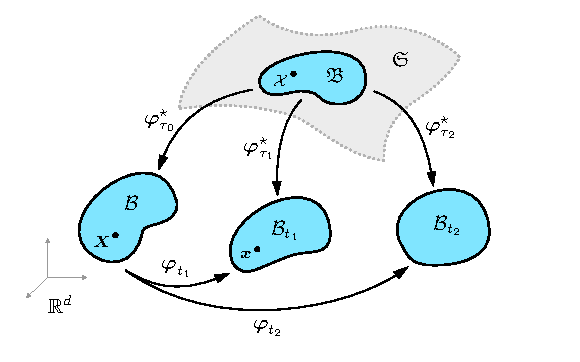
\includegraphics[scale=1.05]{./figures/figure_motion.pdf}
	\caption{Visualized motion of a material body $\mathfrak{B}\!\subset\!\mathfrak{S}$ at different points in time $\tau_{0},\tau_{1},\tau_{2}\!\in\!\mathfrak{T}$. Given an observer $\mathfrak{O}$, each point of the material manifold (real world) $\mathcal{X}\!\in\!\mathfrak{B}$ might be embedded in $\mathbb{R}^{d}$ through a configuration map $\varphi^{\star}_{\tau}$, which depends on the current time $\tau\!\in\!\mathfrak{T}$. Since all these maps are continuously invertible, the observer can arbitrarily chose one of them as the \emph{reference configuration} $\mathcal{B}\!:=\!\mathrm{im}_{\boldsymbol{\varphi}^{\star}_{\tau_{0}}}(\mathfrak{B})$ and identify each of the proceeding configurations based on the composition $\boldsymbol{\varphi}^{\star}_{\tau}\!=\!\boldsymbol{\varphi}_{t}\circ\boldsymbol{\varphi}^{\star}_{\tau_{0}}$. Therein, $\boldsymbol{\varphi}_{t}$ maps referential points $\boldsymbol{X}\!\in\!\mathcal{B}$ towards current positions $\boldsymbol{x}\!\in\!\mathcal{B}_{t}$ at a given observed time $t\!:=\!t(\tau)$.}
	\label{fg:motion}
\end{figure}
Consider some given observer $\mathfrak{O}$ measuring time as $t(\tau)$, the indices within the configuration domains can be simplified even further, so that $\mathcal{B}\!:=\!\mathcal{B}_{\tau_{0}}$ and $\mathcal{B}_{t}\!:=\!\mathcal{B}_{\tau}$ become standard notations throughout this work. Moreover, elements of $\mathcal{B}$ and $\mathcal{B}_{t}$ are denoted as $\boldsymbol{X}$ and $\boldsymbol{x}$, respectively. 
\clearpage
\section{Lists}
A normal list (with itemize).
\begin{itemize}
    \item Item 1
    \item Item 2
    \begin{itemize}
        \item Subitem 1
        \begin{itemize}
            \item Subsubitem 1
        \end{itemize}
        \item Subitem 1
    \end{itemize}
    \item Item 3
\end{itemize}

A numbered list (with enumerate).
\begin{enumerate}
    \item Item
    \item Item
    \begin{enumerate}
        \item Subitem
        \begin{enumerate}
            \item Subsubitem
        \end{enumerate}
        \item Item
    \end{enumerate}
\end{enumerate}

A list with descriptors (with description).
\begin{description}
    \item[Step 1] Step 1 
    \item[Step 2] Step 2 
    \begin{description}
        \item[Substep 1] Substep 1 
            \begin{description}
                \item[Subsubstep 1] Subsubstep 1 
                \item[Subsubstep 2] Subsubstep 2 
            \end{description}
            \item[Substep 2] Substep 2 
    \item[Step 3] Step 3 
    \end{description}
\end{description}

Compact lists sometimes look better (use package paralist).

\begin{compactitem}
    \item Item 1
    \begin{compactitem}
        \item SubItem 1
        \begin{compactitem}
            \item SubSubItem 1
            \item SubSubItem 2
        \end{compactitem}
            \item SubItem 2
    \end{compactitem}
    \item Item 2
\end{compactitem}

Compact list with compactenum
\begin{compactenum}
    \item Item 1
    \begin{compactenum}
        \item SubItem 1
        \begin{compactenum}
            \item SubSubItem 1
            \item SubSubItem 2
        \end{compactenum}
            \item SubItem 2
    \end{compactenum}
    \item Item 2
\end{compactenum}

A compact list with descriptors (compactdesc)
\begin{compactdesc}
    \item[Step 1] Step 1 
    \item[Step 2] Step 2 
    \begin{compactdesc}
        \item[Substep 1] Substep 1 
            \begin{compactdesc}
                \item[Subsubstep 1] Subsubstep 1 
                \item[Subsubstep 2] Subsubstep 2 
            \end{compactdesc}
            \item[Substep 2] Substep 2 
    \item[Step 3] Step 3 
    \end{compactdesc}
\end{compactdesc}

\section{Citations}
Latex provides different citation commands:
\begin{itemize}
    \item cite \cite{Abendroth_ADEM(2004)}
    \item citep \citep{Abendroth_ADEM(2017)}
    \item citet \citet{Abendroth_CMS(2003)}
    \item citealp \citealp{Abendroth_EFM(2006)}
    \item citealt \citealt{Abendroth_IJMS(2024)}
    \item citeauthor \citeauthor{Abendroth_TM(2020)}
    \item citeyear \citeyear{Altenbach2014}
\end{itemize}
